\documentclass[a4paper,10pt]{article}
\setlength{\parindent}{0cm}
\usepackage{amsmath, amssymb, amsthm, mathtools,pgfplots}
\usepackage{graphicx,caption}
\usepackage{verbatim}
\usepackage{venndiagram}
\usepackage[cm]{fullpage}
\usepackage{fancyhdr}
\usepackage{tikz}
\usepackage{listings,url,}
\usepackage{color,enumerate,framed}
\usepackage{color,hyperref}
\definecolor{darkblue}{rgb}{0.0,0.0,0.5}
\hypersetup{colorlinks,breaklinks,
            linkcolor=darkblue,urlcolor=darkblue,
            anchorcolor=darkblue,citecolor=darkblue}

\usepackage{sectsty}
\allsectionsfont{\centering}
%\usepackage[normalem]{ulem}
%\allsectionsfont{\sffamily}
%\sectionfont{\centering\ulemheading{\uuline}}

%\usepackage{tgadventor}
%\usepackage[nohug]{diagrams}
\usepackage[T1]{fontenc}
%\usepackage{helvet}
%\renewcommand{\familydefault}{\sfdefault}
\usepackage{parskip}
%\usepackage{picins} %for \parpic.
%\newtheorem*{notation}{Notation}
%\newtheorem{example}{Example}[section]
%\newtheorem*{problem}{Problem}
\theoremstyle{definition}
%\newtheorem{theorem}{Theorem}
%\newtheorem*{solution}{Solution}
%\newtheorem*{definition}{Definition}
%\newtheorem{lemma}[theorem]{Lemma}
%\newtheorem{corollary}[theorem]{Corollary}
%\newtheorem{proposition}[theorem]{Proposition}
%\newtheorem*{remark}{Remark}
%\setcounter{section}{1}

\newtheorem{thm}{Theorem}[section]
\newtheorem{lemma}[thm]{Lemma}
\newtheorem{prop}[thm]{Proposition}
\newtheorem{cor}[thm]{Corollary}
\newtheorem{defn}[thm]{Definition}
\newtheorem*{examp}{Example}
\newtheorem{conj}[thm]{Conjecture}
\newtheorem{rmk}[thm]{Remark}
\newtheorem*{nte}{Note}
\newtheorem*{notat}{Notation}

%\diagramstyle[labelstyle=\scriptstyle]

\lstset{frame=tb,
  language=Oz,
  aboveskip=3mm,
  belowskip=3mm,
  showstringspaces=false,
  columns=flexible,
  basicstyle={\small\ttfamily},
  breaklines=true,
  breakatwhitespace=true,
  tabsize=3
}


\pagestyle{fancy}




\fancyhead{}
\renewcommand{\headrulewidth}{0pt}

\lfoot{\color{black!60}{\sffamily Zhangsheng}}
\cfoot{}
\cfoot{\color{black!60}{\sffamily Last modified: \today}}
\rfoot{\color{black!60}{\sffamily\thepage}}



\begin{document}
\begin{flushright}
Zhangsheng Lai
\end{flushright}

This discussion attempts to analyse the cooperation and competition problem using the congestion games approach. The idea was motivated by the opting out example that was discussed in class as it was seen that the structure has some similarities to the problem we are trying to understand here.

\newdimen\R
\R=2cm
\begin{figure}[h]
\centering
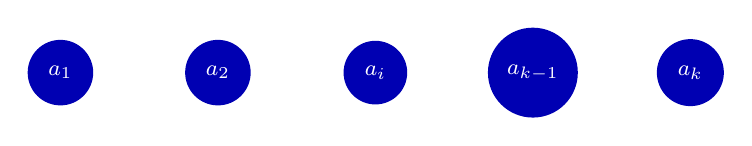
\begin{tikzpicture}[scale=1,draw=black!50,>=latex]
	\tikzstyle{neuron}=[circle,fill=black!25,
	minimum size=1pt,
	inner sep=5pt
	]
	\tikzstyle{m}=[neuron, fill=blue!70!black];
	\tikzstyle{n}=[neuron, fill=red!70!white];

\node[m](a1) at (-4,0){\footnotesize {\color{white}$a_{1}$}};
\node[m](a1) at (-2,0){\footnotesize {\color{white}$a_2$}};
\node[m](a1) at (0,0){\footnotesize {\color{white}$a_i$}};
\node[m](a1) at (2,0){\footnotesize {\color{white}$a_{k-1}$}};
\node[m](a1) at (4,0){\footnotesize {\color{white}$a_k$}};

\end{tikzpicture}
\end{figure}

%	\newdimen\R
%\R=2cm
%\begin{figure}[h]
%	\centering
%	\begin{tikzpicture}[scale=1,draw=black!50,>=latex]
%	\tikzstyle{neuron}=[circle,fill=black!25,minimum size=15pt,inner sep=0pt]
%	\tikzstyle{m}=[neuron, fill=blue!70!black];
%	\tikzstyle{n}=[neuron, fill=red!70!white];
%%	\foreach \x in {1,2,3}{
%%	\node[m,yshift=\x*2 cm](s-\x) at (\x*2-2*2,1){\footnotesize {\color{white}$s_{\x}$}};
%%	\node[n,yshift=\x*2 cm](t-\x) at (\x*2-2*2,-1){\footnotesize {\color{white}$t_{\x}$}};
%%	}
%%	
%	\node[m,yshift=2 cm](s-1) at (-2,1){\footnotesize {\color{white}$v^s_1$}};;
%	\node[m,yshift=4 cm](s-2) at (0,1){\footnotesize {\color{white}$v^s_2$}};
%	\node[m,yshift=6 cm](s-3) at (2,1){\footnotesize {\color{white}$v^s_3$}};
%	\node[n,yshift=2 cm](t-1) at (-2,-1){\footnotesize {\color{white}$v^t_1$}};
%	\node[n,yshift=4 cm](t-2) at (0,-1){\footnotesize {\color{white}$v^t_2$}};
%	\node[n,yshift=6 cm](t-3) at (2,-1){\footnotesize {\color{white}$v^t_3$}};
%	\foreach \x in {1,2,3}{
%	\draw[->,color=black,thick] (s-\x) -- (t-\x);
%	\draw[->,thick,dashed] (s-\x) edge[bend right] (t-\x);
%	\draw[->,thick,dashed] (s-\x) edge[bend left] (t-\x);
%	}
%	\draw[->,thick,dashed] (s-1) edge[bend left] (s-2);
%	\draw[->,thick,dashed] (s-1) edge[bend left] (s-3);
%	\draw[->,thick,dashed] (s-2) edge (s-3);
%	\draw[->,thick,dashed] (s-2) edge (s-1);
%	\draw[->,thick,dashed] (s-3) edge[bend left] (s-2);
%	\draw[->,thick,dashed] (s-3) edge[bend left] (s-1);
%	\end{tikzpicture}
%	\caption{Office game seen as a routing game with 3 agents}
%	\label{fig:officerouting}
%\end{figure}
%


\end{document}